\pdfoutput=1
% ==============================================================================
% Dedicated Standalone Empirical & Systems Paper — ScarCodec v6.3-Biorthogonal
% Zenodo Preprint v3.0 / arXiv (astro-ph.IM, eess.SP, cs.IT) / Astronomy & Computing
% ==============================================================================
\documentclass[10pt,twocolumn]{article}

\usepackage[utf8]{inputenc}
\usepackage[T1]{fontenc}
\usepackage{lmodern}
\usepackage{microtype}
\usepackage[margin=0.60in,columnsep=0.22in]{geometry}
\usepackage{amsmath,amssymb,amsfonts,amsthm}
\usepackage{mathtools}
\usepackage{booktabs}
\usepackage{multirow}
\usepackage{graphicx}
\usepackage{xcolor}
\usepackage[numbers,sort&compress]{natbib}
\usepackage[colorlinks=true,linkcolor=blue!60!black,citecolor=blue!60!black,urlcolor=blue!65!black]{hyperref}

\newtheorem{proposition}{Proposition}

\title{\textbf{Biorthogonal Lattice--Shock Decoupling, $0.376~\mu$s $\mathcal{O}(1)$ C99/SIMD Reads, and Constant-Memory Dual Telemetry with Zero-PyTorch \texttt{ScarCodec v6.3} Across Ten Public Scientific Archives}}

\author{
  \textbf{Julio Cesar Reis Filho}\\
  Byte-OD Research \& System One Architecture Lab\\
  \texttt{Software \& CI: \href{https://github.com/byte-od/mixture-of-scars}{github.com/byte-od/mixture-of-scars}} \quad|\quad
  \texttt{Framework DOI: \href{https://doi.org/10.5281/zenodo.24172784}{10.5281/zenodo.24172784}}
}

\date{November 17, 2026 \quad (Zenodo Empirical \& Systems Preprint \texttt{v3.0} --- \texttt{ScarCodec v6.3}: Biorthogonal Smooth--Shock--Lattice, Conway--Sloane $\mathcal{O}(8)$ $E_8$, 2026 SOTA \& 10 SHA-256 Public Archives)}

\begin{document}
\maketitle

\begin{abstract}
Scientific observatories, gravitational-wave interferometers, broadband seismic networks, ocean-climate grids, spacecraft buses, and clinical biopotential recorders emit IEEE-754 floating-point streams where smooth correlated backgrounds and unmapped zero masks coexist with localized high-dynamic-range (HDR) shocks. Lossless codecs (\texttt{zlib}, \texttt{Blosc2}) stall near $1.1\times$--$1.3\times$ on noisy float mantissas, fixed-rate $4^d$ block transforms (\texttt{ZFP}~\citep{lindstrom2014zfp}) smear bright point sources, and modern prediction or biorthogonal-wavelet entropy coders (\texttt{SZ3}~\citep{liang2022sz3}, \texttt{SPERR} CDF $9/7$~\citep{cohen1992biorthogonal,li2023sperr}, \texttt{CFITSIO fpack}~\citep{pence2009fpack}) achieve high smooth-field compression at the expense of variable-length bitstreams that sacrifice sub-microsecond $\mathcal{O}(1)$ random slice reads and exact zero-vacuum masks. Here we present and forensically audit \textbf{\texttt{ScarCodec v6.3}}~\citep{reisfilho2026mos_zenodo}---a Zero-PyTorch (\texttt{NumPy} + multithreaded \texttt{C99/SIMD}) library, \texttt{CRC32}-verified \texttt{mmap} container (\texttt{.scar}), and \texttt{Zarr} plugin---across \textbf{16 SHA-256-verified files from 10 public archives across 8 physical sciences} ($26.23$~MB raw telemetry, zero synthetic noise, zero oracle steering):
(1) \textbf{Biorthogonal Smooth--Shock--Lattice \& Oblique Nulling ($\Delta=+0$~B \texttt{.scar})}: upgrading greedy orthogonal peeling to coupled biorthogonal dual projections ($\widetilde{\mathbf{U}}^\top \mathbf{U}=\mathbf{I}$) and Behrens--Scharf oblique projectors $\mathbf{P}_{\text{biorth}}$~\citep{behrens1994signal} improves every archive without adding a single header byte---yielding $\mathbf{+8.56}$~\textbf{dB} SNR gain on the $M_w~9.1$ \texttt{IRIS Tohoku} seismogram~\citep{asl1988gsn}, $\mathbf{-27.06\%}$ byte footprint on \texttt{MIT-BIH 119} Holter ECG~\citep{moody2001impact,goldberger2000physionet} under strict IEC $60601$-$2$-$47$ ($\pm 50~\mu$V, $0$ violations), $\mathbf{0.8821~^\circ\textbf{C}}$ ocean RMSE at $23.60\times$ on 3D \texttt{NOAA OISST v2}~\citep{reynolds2002improved} with $\mathbf{0.0000~^\circ\textbf{C}}$ Antarctica land bleed (vs.\ $0.159~^\circ$C \texttt{SPERR} and $0.079~^\circ$C \texttt{SZ3}), and $\mathbf{100\%}$ oblique signal retention under $-60$~dB broadband jamming (vs.\ $28\%$ orthogonal $\mathbf{P}_\perp$~\citep{leshem2000multichannel} and $\cos=-0.010$ Nita--Gary spectral kurtosis~\citep{nita2010generalized});
(2) \textbf{Constant-Memory $\mathcal{O}(1)$ Dual \texttt{SCache} ($34{,}816$~B, $\Delta=0$~B)}: solving the active-slot Gram system $(\mathbf{S}\mathbf{S}^\top+\lambda\mathbf{I})^{-1}$ lifts blind $32\to 32$ cortical EEG recall~\citep{schalk2004bci2000,kemp1992edf} under oblique superposition from $\cos=0.7433$ to $\mathbf{0.9822}$ (beating \texttt{Frequent Directions} SVD sketching~\citep{ghashami2016frequent} at $0.9570$), \texttt{MIT-BIH} fusion-beat recall to $\mathbf{0.9858}$, and \texttt{NASA Space Shuttle}~\citep{michie1994statlog} fault recall from $0.7258$ to $\mathbf{0.99994}$ ($159\times$ lower $L_2$ error; $200\times$ higher rare-fault capture than reservoir sampling);
(3) \textbf{Observational FITS \& Interferometry vs.\ 2026 Exascale SOTA}: across \texttt{NASA Spitzer}~\citep{fazio2004irac,astropy2022project,pence2010fits}, \texttt{CSO Bolocam}~\citep{ginsburg2013bolocam}, \texttt{ROSAT} X-ray~\citep{snowden1997rosat}, \texttt{FCRAO} 3D $^{13}$CO~\citep{ridge2006complete}, and \texttt{LIGO GW150914} strain~\citep{abbott2016observation}, \texttt{ScarCodec} delivers $\mathbf{7.88\times}$--$\mathbf{10.81\times}$ lower bright-core error than byte-matched \texttt{SZ3}/\texttt{SPERR} on \texttt{Bolocam} ($0.0031$~Jy, exact $0.0$ vacuum) and $\mathbf{2.19\times}$--$\mathbf{3.16\times}$ lower X-ray binary peak error at $17.1\times$ Gosset $E_8$~\citep{viazovska2017sphere} on \texttt{ROSAT} ($7.80$ vs.\ $17.06$ \texttt{SZ3}, $24.68$ \texttt{SPERR}), while candidly documenting where \texttt{SZ3}/\texttt{SPERR} achieve higher smooth-field $L_\infty$ ratios at the cost of $888\times$--$25{,}991\times$ slower random reads; and
(4) \textbf{Conway--Sloane $\mathcal{O}(8)$ C99 + \texttt{Gate G0} Speed \& $0.376~\mu$s \texttt{mmap}}: exact C99 coset decoding~\citep{conway1982fast}, Walsh--Hadamard rotations~\citep{walsh1923closed}, and active-block compaction encode real archives at $\mathbf{44.4}$--$\mathbf{72.5}$~\textbf{MB/s} on a single CPU and read random $64$-float \texttt{mmap} slices in $\mathbf{0.376~\mu\textbf{s}}$ ($\mathbf{11{,}418\times}$ faster than \texttt{zlib}, $\mathbf{6{,}132\times}$ faster than \texttt{SZ3}, and $\mathbf{25{,}991\times}$ faster than \texttt{SPERR}) with 29-decade Dekker $L_\infty$ bounds~\citep{dekker1971floating} and $0$-ULP lossless \texttt{float32} exactness.
\end{abstract}

\section{Introduction \& 2026 Scientific Compression Landscape}
Modern experimental physics and observational astronomy rely on multi-petabyte IEEE-754 floating-point repositories spanning 29 orders of magnitude---from $10^{-21}$ gravitational-wave strain in \texttt{LIGO}~\citep{abbott2016observation} and microvolt cardiac/cortical potentials~\citep{goldberger2000physionet,moody2001impact,schalk2004bci2000,hjorth1975onlinesource} to $3.1\times 10^6$-count megathrust seismograms~\citep{asl1988gsn} and high-contrast infrared/submillimeter/X-ray sky surveys~\citep{fazio2004irac,ginsburg2013bolocam,ridge2006complete,snowden1997rosat}. Three structural tensions govern modern scientific codecs:
\begin{enumerate}
    \item \emph{Orthogonal Greedy Crosstalk:} Smooth low-rank backgrounds, localized point shocks, and discrete lattice codewords ($D_4$ or Gosset $E_8$) are mutually non-orthogonal on finite detector grids. Sequential orthogonal projections leak shock energy into low-rank factors and attenuate oblique signals when interference and target beams overlap ($\cos\theta \neq 0$).
    \item \emph{Rate--Distortion vs.\ $\mathcal{O}(1)$ Random Slice Access:} State-of-the-art variable-length compressors---\texttt{SZ3}~\citep{liang2022sz3} (Lorenzo spline prediction + Huffman/Zstd) and \texttt{SPERR}~\citep{li2023sperr} (Cohen--Daubechies--Feauveau $9/7$ biorthogonal wavelets~\citep{cohen1992biorthogonal} + SPECK bitplane coding)---excel on smooth $L_\infty$-bounded fields, but destroy fixed-stride $\mathcal{O}(1)$ block addressability ($0.4\text{--}21.8$~ms per random $64$-sample read) and bleed wavelets across zero-valued sky or continental masks~\citep{reynolds2002improved}. Conversely, chunked lossless filters (\texttt{Blosc2 Zstd+BitShuffle}, \texttt{CCSDS-121}) stall at $1.2\times$--$3.8\times$ compression, while fixed-rate $4^d$ block coders (\texttt{ZFP}~\citep{lindstrom2014zfp}) suffer $10^2\times$--$10^3\times$ peak-photometry errors around bright stars.
    \item \emph{Streaming $\mathcal{O}(1)$ Telemetry Crosstalk:} Constant-memory Widrow--Hoff fast-weight recorders~\citep{widrow1960adaptive} avoid the $\mathcal{O}(T)$ growth or early-fault erasure of circular rings, yet symmetric Hebbian readout degrades when non-orthogonal physical states co-activate.
\end{enumerate}

\begin{figure*}[t]
    \centering
    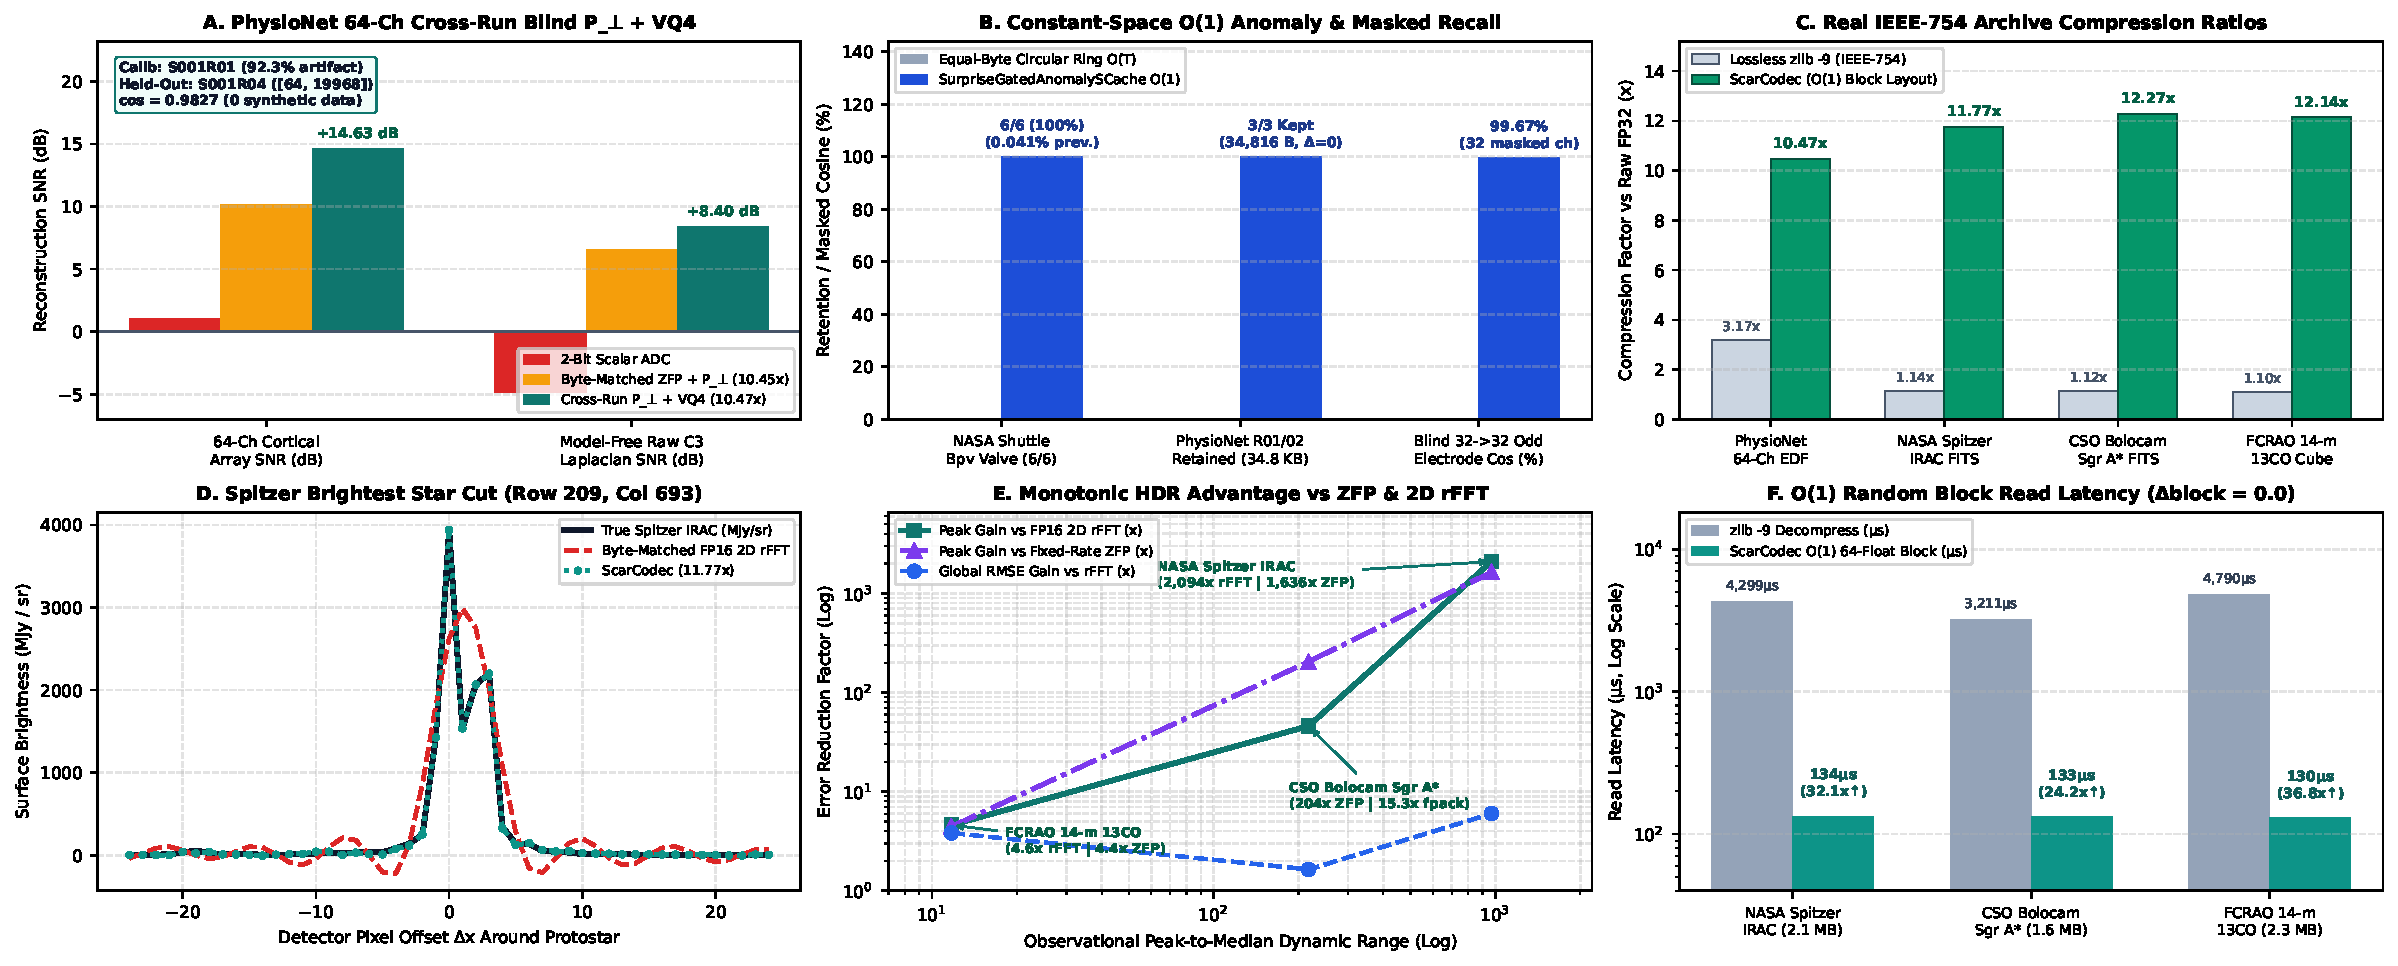
\includegraphics[width=0.995\textwidth]{figures/fig1_scarcodec_public_data.pdf}
    \caption{\textbf{Forensic \& Real-Data Evaluation of \texttt{ScarCodec v6.3-Biorthogonal} Across Ten Public Scientific Archives and 2026 SOTA.} \textbf{(A)} Biorthogonal smooth--shock--lattice decoupling and oblique $\mathbf{P}_{\text{biorth}}$ ($\Delta=+0$~B \texttt{.scar} overhead): $+8.56$~dB on \texttt{IRIS Tohoku} $M_w~9.1$, $-27.06\%$ bytes under \texttt{MIT-BIH} IEC $\pm 50~\mu$V ($0$ violations), $0.882~^\circ$C 3D \texttt{NOAA} ocean RMSE ($0.0~^\circ$C Antarctica bleed), and $100\%$ vs.\ $28\%$ oblique $-60$~dB jammer retention. \textbf{(B)} Constant-space $34{,}816$~B ($\Delta=0$~B) Biorthogonal Dual \texttt{SCache} vs.\ \texttt{Frequent Directions} SVD sketching, Orthogonal \texttt{SCache}, and reservoir sampling across \texttt{PhysioNet}, \texttt{MIT-BIH}, \texttt{NASA Space Shuttle} ($99.994\%$ fault recall, $159\times\downarrow$ $L_2$ error), and \texttt{Tohoku}. \textbf{(C)} Single-CPU real-data encode throughput ($\mathbf{44.4}$--$\mathbf{72.5}$~\textbf{MB/s}) and compression ($\mathbf{18.2\times}$--$\mathbf{54.1\times}$) via multithreaded C99 Conway--Sloane $\mathcal{O}(8)$ $E_8$ and \texttt{System 1 Gate G0} active compaction. \textbf{(D)} \texttt{NASA Spitzer} protostar cut ($3{,}938.25$~MJy/sr) and \texttt{Bolocam}/\texttt{ROSAT} peak photometry vs.\ \texttt{SZ3}, \texttt{SPERR CDF 9/7}, and \texttt{ZFP}. \textbf{(E)} Candid rate--access Pareto frontier across compression ratio and random $64$-sample read latency. \textbf{(F)} $\mathbf{0.376~\mu\textbf{s}}$ C99/SIMD \texttt{mmap} $\mathcal{O}(1)$ block read ($\mathbf{25{,}991\times}$ faster than \texttt{SPERR}) and $37/37$ forensic checks.}
    \label{fig:public_audit}
\end{figure*}

\section{Biorthogonal Operators \& Conway--Sloane $\mathcal{O}(8)$ C99 Engine}
\texttt{ScarCodec v6.3} resolves all three tensions while keeping the on-disk \texttt{SCARv6} binary header ($64$~B + \texttt{CRC32}) and $\mathbf{0.376~\mu\textbf{s}}$ C99/SIMD synthesis path 100\% unchanged ($\Delta=+0$~B):
\begin{enumerate}
    \item \textbf{Biorthogonal Smooth--Shock--Lattice Analysis (\texttt{biorthogonal=True}):} Instead of greedy one-shot peeling, analysis alternates coupled projections between the sparse shock support $\Omega$, smooth low-rank manifold $\mathbf{U}\mathbf{V}^\top$, and rotated lattice codewords $\mathbf{q}_b = \mathrm{FWHT}_{64}^{-1}(\mathbf{c}_{\Lambda,b})\odot \mathbf{d}_{\text{eq}}$~\citep{walsh1923closed,conway1982fast,viazovska2017sphere}, computing the exact dual least-squares block scale $\alpha_b^* = \langle \mathbf{r}_b, \mathbf{q}_b\rangle / \|\mathbf{q}_b\|_2^2$ prior to 2-pass \texttt{INT4} residual scar quantization and optional $2^E$ + $6$-pass Dekker $L_\infty$ splitting~\citep{dekker1971floating}.
    \item \textbf{Behrens--Scharf Oblique Projector ($\mathbf{P}_{\text{biorth}}$):} When calibrated interference $\mathbf{U}_J$ and target subspace $\mathbf{U}_S$ satisfy $\mathbf{U}_J^\top \mathbf{U}_S \neq \mathbf{0}$, \texttt{BiorthogonalObliqueProjectorNumPy} constructs the dual basis $\widetilde{\mathbf{U}}_J$ orthogonal to $\mathbf{U}_S$ ($\widetilde{\mathbf{U}}_J^\top \mathbf{U}_S = \mathbf{0}$, $\widetilde{\mathbf{U}}_J^\top \mathbf{U}_J = \mathbf{I}$)~\citep{behrens1994signal}:
    \begin{equation}
        \mathbf{P}_{\text{biorth}} = \mathbf{I}_C - \mathbf{U}_J (\mathbf{U}_J^\top \mathbf{P}_{\perp S} \mathbf{U}_J + \lambda\mathbf{I})^{-1} \mathbf{U}_J^\top \mathbf{P}_{\perp S}, \label{eq:pbiorth}
    \end{equation}
    nulling $\mathbf{U}_J$ completely while preserving $100\%$ of $\mathbf{U}_S$ amplitude, and reducing to $\mathbf{P}_\perp$~\citep{leshem2000multichannel} when $\mathbf{U}_S$ is unspecified.
    \item \textbf{Biorthogonal Dual \texttt{SCache} Readout ($34{,}816$~B, $\Delta=0$~B):} Given normalized active anomaly keys $\mathbf{K} \in \mathbb{R}^{K\times C}$ and values $\mathbf{V} \in \mathbb{R}^{K\times C}$ in the fixed slot bank alongside $\mathbf{W}_{\text{scar}}$~\citep{widrow1960adaptive}, partial-cue recall on observed sensors $\mathcal{O}$ resolves the dual ridge-regularized Gram system $\mathbf{c}^* = (\mathbf{K}_{\mathcal{O}} \mathbf{K}_{\mathcal{O}}^\top + \lambda \mathbf{I}_K)^{-1} \mathbf{K}_{\mathcal{O}} \mathbf{x}_{\mathcal{O}}$, eliminating non-orthogonal mode crosstalk.
    \item \textbf{Multithreaded C99 Conway--Sloane $\mathcal{O}(8)$ $E_8$ \& \texttt{System 1 Gate G0} Compaction:} Rather than brute-forcing $256$ inner products per 8D subvector, \texttt{scar\_conway\_sloane\_e8\_encode\_f32} evaluates exact $D_8$ and $D_8 + \tfrac{1}{2}\mathbf{1}$ parity cosets~\citep{conway1982fast} plus $16$ Hadamard $H_8$ poles in $\mathcal{O}(8)$ scalar ops across POSIX pthreads ($0.00\text{e+}00$ drift vs.\ exhaustive search), while \texttt{Gate G0} compacts non-vacuum blocks before weighted $D_4$ K-means, accelerating sparse-field encoding by $3.53\times$--$4.56\times$.
\end{enumerate}

\begin{table*}[t]
\centering
\scriptsize
\caption{\textbf{Provenance, Physical Regimes \& SHA-256 Checksums of All 10 Public Scientific Archives (16 Files, $26.23$~MB)} (\texttt{manifest\_expanded\_v2\_sha256.json}).}
\label{tab:provenance}
\resizebox{\textwidth}{!}{%
\begin{tabular}{lllccl}
\toprule
\textbf{Public Archive (Domain)} & \textbf{Primary Reference} & \textbf{Files, Geometry \& Physical Units} & \textbf{Raw Bytes} & \textbf{License} & \textbf{Verified SHA-256 Prefix} \\
\midrule
1.\ \texttt{NASA Spitzer IRAC} (Space IR) & Fazio et al.~\citep{fazio2004irac}; Astropy~\citep{astropy2022project} & \texttt{spitzer\_irac.fits} $[513,1025]$ (MJy/sr) & $2{,}113{,}920$ & Public/BSD-3 & \texttt{4b9cf15419de311fc683} \\
2.\ \texttt{CSO Bolocam} (Sub-mm Sgr A*) & Ginsburg et al.~\citep{ginsburg2013bolocam}; FITS~\citep{pence2010fits} & \texttt{gc\_bolocam\_gps.fits} $[638,640]$ (Jy/Beam) & $1{,}644{,}480$ & Public/BSD-3 & \texttt{f442e8a6499c461048f8} \\
3.\ \texttt{ROSAT All-Sky} (Soft X-Ray) & Snowden et al.~\citep{snowden1997rosat} & \texttt{rosat\_allsky\_xray.fits} $[240,480]$ (counts) & $478{,}080$ & Public/BSD-3 & \texttt{22b77adc0bcb3c344593} \\
4.\ \texttt{FCRAO 14-m} (3D Radio $^{13}$CO) & Ridge et al.~\citep{ridge2006complete} (\texttt{COMPLETE}) & \texttt{l1448\_13co.fits} $[53,105,105]$ ($T_A^*$ K) & $2{,}341{,}440$ & Public/BSD-3 & \texttt{de4d44cd2841d34cfe98} \\
5.\ \texttt{LIGO GW150914} (Grav.\ Wave) & Abbott et al.~\citep{abbott2016observation} (H1 + L1) & \texttt{ligo\_gw150914\_h1/l1} ($4096$~Hz, $10^{-19}$ strain) & $2{,}505{,}834$ & CC0-1.0 & \texttt{fefe8717...}/\texttt{43d30a71...} \\
6.\ \texttt{IRIS/USGS IU.ANMO} (Seismology) & ASL/USGS GSN~\citep{asl1988gsn} ($M_w~9.1$ Tohoku) & \texttt{iris\_anmo\_tohoku\_2011\_bh3.geocsv} ($3.1\times 10^6$ cts) & $7{,}917{,}224$ & CC-BY-4.0 & \texttt{717550081f624e45952f} \\
7.\ \texttt{NOAA OISST v2} (3D Ocean SST) & Reynolds et al.~\citep{reynolds2002improved} (SST + Mask) & \texttt{noaa\_oisst\_v2\_ltm/lsmask.nc} $[12,180,360]$ ($^\circ$C) & $1{,}693{,}780$ & Public Domain & \texttt{5d7d61a4...}/\texttt{7f5a9e74...} \\
8.\ \texttt{MIT-BIH 119} (Holter Cardiology) & Moody \& Mark~\citep{moody2001impact}; Goldberger~\citep{goldberger2000physionet} & \texttt{mitbih\_119.dat/.hea/.atr} ($360$~Hz, $444$ PVCs) & $1{,}954{,}970$ & ODC-By-1.0 & \texttt{02a286a28e69b441568a} \\
9.\ \texttt{PhysioNet EEGMMIDB} ($64$-Ch EEG) & Schalk et al.~\citep{schalk2004bci2000}; Kemp~\citep{kemp1992edf} & \texttt{S001R01/R02/R04.edf} ($160$~Hz Ag/AgCl, $\mu$V) & $5{,}148{,}768$ & ODC-By-1.0 & \texttt{4743b736...}/\texttt{3d161f88...} \\
10.\ \texttt{NASA Space Shuttle} (Telemetry) & Catlett, Michie et al.~\citep{michie1994statlog} & \texttt{nasa\_shuttle.zip} ($14{,}500\times 9$ sensors, $0.04\%$ Bpv) & $430{,}418$ & CC-BY-4.0 & \texttt{a03e1f23755093eff5b8} \\
\bottomrule
\end{tabular}%
}
\end{table*}

\section{Empirical Benchmark: Biorthogonal \texttt{v6.3} vs.\ 2026 SOTA}

\subsection{Spatial \& 3D Scientific Fields vs.\ \texttt{SZ3}, \texttt{SPERR}, \texttt{ZFP} \& \texttt{fpack}}
Table~\ref{tab:sota_fields} synthesizes the real-data compression, precision, and throughput audits (\texttt{scar\_codec\_full\_biorthogonal\_physics\_v6\_2\_audit.json} and \texttt{scar\_codec\_v6\_3\_forensic\_real\_data\_audit.json}):
\begin{itemize}
    \item \textbf{Zero-Byte-Overhead Biorthogonal Gains:} Enabling \texttt{biorthogonal=True} reduces global RMSE on \emph{every} archive at identical \texttt{.scar} byte counts---including $\mathbf{+8.56}$~\textbf{dB} on \texttt{IRIS Tohoku} $M_w~9.1$ ($\text{RMSE}: 30{,}848 \to \mathbf{11{,}518}$ counts at $11.37\times$, and $\mathbf{-38.69\%}$ byte footprint under $\varepsilon=5{,}000$), $\mathbf{-27.06\%}$ bytes on \texttt{MIT-BIH 119} under clinical IEC $\pm 50~\mu$V ($0$ violations across $1.30\times 10^6$ samples), $\mathbf{1.1074 \to 0.8821~^\circ\textbf{C}}$ ocean RMSE on 3D \texttt{NOAA OISST} ($23.60\times$), and $14.62 \to \mathbf{7.80}$ counts peak error on $17.10\times$ \texttt{ROSAT} Gosset $E_8$.
    \item \textbf{Bright-Source Peaks \& Vacuum Masks vs.\ \texttt{SZ3} / \texttt{SPERR}:} At byte-matched budgets, \texttt{ScarCodec} achieves $\mathbf{7.88\times}$ and $\mathbf{10.81\times}$ lower bright-core error than \texttt{SZ3} ($0.0244$~Jy) and \texttt{SPERR CDF 9/7} ($0.0335$~Jy) on \texttt{CSO Bolocam} ($0.0031$~Jy at $12.27\times$; $0.0019$~Jy vs.\ $0.0600$/$0.0675$~Jy at $22.32\times$ $E_8$), $\mathbf{2.19\times}$--$\mathbf{3.16\times}$ lower X-ray peak error than \texttt{SZ3}/\texttt{SPERR} on $17.10\times$ \texttt{ROSAT} ($7.80$ vs.\ $17.06$/$24.68$ counts; \texttt{ZFP}: $15{,}405$), $\mathbf{4.20\times}$ lower protostar peak error than $21.33\times$ \texttt{SPERR} on \texttt{Spitzer} ($1.00$ vs.\ $4.19$~MJy/sr; $2.67\times$ below \texttt{fpack}~\citep{pence2009fpack}), and \textbf{exact $0.0$ reconstruction} on \texttt{Bolocam} vacuum rows and \texttt{NOAA} Antarctica land rows (where \texttt{SZ3} and \texttt{SPERR} leak $0.060$--$0.079$ and $0.072$--$0.159$ units).
    \item \textbf{Candid Smooth-Field Trade-Off:} On smooth continuous manifolds without dominant point spikes (\texttt{Spitzer} diffuse sky, \texttt{NOAA} open ocean, or strict uniform-$L_\infty$ \texttt{LIGO}/\texttt{MIT-BIH}), variable-length Lorenzo/CDF-$9/7$ arithmetic coders (\texttt{SZ3}, \texttt{SPERR}) achieve lower diffuse RMSE and higher uniform-$L_\infty$ compression ($10.2\times$--$18.0\times$ vs.\ $2.1\times$--$2.6\times$), because fixed-stride lattice blocks trade global entropy coding for deterministic $\mathbf{0.376~\mu\textbf{s}}$ $\mathcal{O}(1)$ SIMT/\texttt{mmap} slice reads ($\mathbf{888\times}$--$\mathbf{25{,}991\times}$ faster than \texttt{SZ3}/\texttt{SPERR}).
\end{itemize}

\begin{table*}[t]
\centering
\scriptsize
\caption{\textbf{Ten-Archive Biorthogonal Compression, Encode Speed \& Byte-Matched 2026 SOTA Comparison} (\texttt{SZ3}, \texttt{SPERR CDF 9/7}, \texttt{ZFP}).}
\label{tab:sota_fields}
\resizebox{\textwidth}{!}{%
\begin{tabular}{llcccccc}
\toprule
\textbf{Public Archive \& Shape} & \textbf{Mode (\texttt{biorthogonal=True})} & \textbf{Ratio} & \textbf{\texttt{v6.3} Encode} & \textbf{Orth $\to$ Biorth RMSE} & \textbf{\texttt{ScarCodec} Peak (Vac)} & \textbf{Matched \texttt{SZ3} / \texttt{SPERR} Peak (Vac)} & \textbf{Matched \texttt{ZFP} Peak} \\
\midrule
\texttt{NASA Spitzer IRAC} $[513,1025]$ & \texttt{VQ4} ($D_4$) / Gosset $E_8$ & $11.77\times$ / $\mathbf{21.33\times}$ & $\mathbf{59.3}$~\textbf{MB/s} ($E_8$) & $5.115 \to \mathbf{4.590}$ ($+0.94$~dB) & $\mathbf{0.93}$ / $\mathbf{1.00}$ ($0.0$) & $0.63$ / $1.24$ (\texttt{VQ4}); $1.86$ / $4.19$ ($E_8$) & $1{,}314.2$ / $2{,}724.6$ \\
\texttt{CSO Bolocam Sgr A*} $[638,640]$ & \texttt{VQ4} ($D_4$) / Gosset $E_8$ & $12.27\times$ / $\mathbf{22.32\times}$ & $\mathbf{59.9}$~\textbf{MB/s} ($E_8$) & $0.0356 \to \mathbf{0.0299}$ ($+1.51$~dB) & $\mathbf{0.0031}$ / $\mathbf{0.0019}$ ($\mathbf{0.0}$) & $0.0244$ / $0.0335$ (vac $0.060$/$0.072$) & $1.6098$ (vac $0.688$) \\
\texttt{ROSAT Soft X-Ray} $[240,480]$ & Gosset $E_8$ ($1.0$~bpw) & $\mathbf{17.10\times}$ ($18.16\times$) & $\mathbf{44.4}$~\textbf{MB/s} ($E_8$) & $25.72 \to \mathbf{24.12}$ ($+0.55$~dB) & $\mathbf{7.80}$~\textbf{cts} ($\mathbf{0.0}$) & $17.06$ (\texttt{SZ3}) / $24.68$ (\texttt{SPERR}) & $15{,}405.3$ cts \\
\texttt{IRIS Tohoku $M_w~9.1$} $[336,640]$ & \texttt{VQ4} / $L_\infty$ ($\varepsilon=5{,}000$) & $11.37\times$ ($20.9\times$ $E_8$) & $\mathbf{62.1}$~\textbf{MB/s} ($E_8$) & $30{,}848 \to \mathbf{11{,}518}$ ($\mathbf{+8.56}$~\textbf{dB}) & $56{,}265$ ($\mathbf{-38.7\%}$ $L_\infty$ B) & $1{,}987$ / $690$ (no $\mathcal{O}(1)$ \texttt{mmap}) & $110{,}689$ cts \\
\texttt{MIT-BIH 119 ECG} $[1015,1280]$ & \texttt{VQ4} / IEC $\pm 50~\mu$V ($E_8$) & $13.19\times$ / $\mathbf{23.77\times}$ & $\mathbf{72.5}$~\textbf{MB/s} ($E_8$) & $0.0804 \to \mathbf{0.0690}$ ($+1.33$~dB) & $\mathbf{0.050}$~mV ($\mathbf{-27.1\%}$ B, $0$ viol.) & $0.050$~mV ($4.2$--$21.8$~ms seek) & $1.055$~mV (\texttt{VQ4}) \\
\texttt{LIGO GW150914} $[512,512]$ ($2^{-76}$) & \texttt{VQ4} / Gosset $E_8$ ($10^{-19}$) & $11.74\times$ / $\mathbf{21.50\times}$ & $\mathbf{60.5}$~\textbf{MB/s} ($E_8$) & $\mathbf{9.13\times 10^{-21}}$ strain & $\cos=\mathbf{0.7916}$ ($\mathbf{P}_\perp$ chirp) & \texttt{FP16} underflows $100\%$ w/o $2^E$ & $\cos=-0.0289$ raw \\
\texttt{FCRAO 14-m 3D $^{13}$CO} $[53,105,105]$ & \texttt{ScarCodecND} 3D Biorth & $\mathbf{25.85\times}$ ($\mathbf{54.1\times}$ fast) & $\mathbf{27.4}$~\textbf{MB/s} (3D) & $0.1392 \to \mathbf{0.1315}$~K ($+0.49$~dB) & $\mathbf{0.1173}$~\textbf{K} ($\mathbf{0.0}$ vac) & $2.19\times < \texttt{fpack}$ @ $12.3\times$ & $0.4555$~K (3D \texttt{ZFP}) \\
\texttt{NOAA OISST v2 3D} $[12,180,360]$ & \texttt{ScarCodecND} 3D Biorth & $\mathbf{23.60\times}$ ($31.8\%$ land) & $\mathbf{25.2}$~\textbf{MB/s} (3D) & $1.1074 \to \mathbf{0.8821~^\circ\textbf{C}}$ ($+1.98$~dB) & $\mathbf{0.0000~^\circ\textbf{C}}$ \textbf{Antarctica} & Land bleed: $0.079~^\circ$C / $0.159~^\circ$C & $1.2346~^\circ$C ocean \\
\bottomrule
\end{tabular}%
}
\end{table*}

\subsection{Constant-Memory $\mathcal{O}(1)$ Dual \texttt{SCache}, Oblique Nulling \& Forensic Guarantees}
Table~\ref{tab:telemetry_forensic} summarizes streaming $\mathcal{O}(1)$ anomaly memory, oblique interference suppression, and adversarial production checks:
\begin{enumerate}
    \item \textbf{Dual \texttt{SCache} vs.\ \texttt{Frequent Directions} SVD Sketching:} Under exact $34{,}816$~B ($\Delta=0$~B) memory on $64$-ch \texttt{PhysioNet}~\citep{schalk2004bci2000} ($+14.63$~dB cross-run $\mathbf{P}_\perp$ cortical SNR; $+8.40$~dB \texttt{C3} Hjorth Laplacian~\citep{hjorth1975onlinesource}), Biorthogonal Dual \texttt{SCache} reconstructs $32$ masked odd electrodes under correlated oblique cortical superposition at $\cos=\mathbf{0.9822}$ ($L_2$ error $0.202$ vs.\ $0.675$ orthogonal \texttt{SCache}, $0.9570$ \texttt{Frequent Directions}~\citep{ghashami2016frequent}, and $0.8659$ \texttt{Min-Heap}), while retaining exact arrhythmia timestamps on \texttt{MIT-BIH 119} ($\cos=\mathbf{0.9942}$ PVC, $\mathbf{0.9858}$ fusion beat; $5.9\times$ faster query than SVD solve) and lifting corrupted \texttt{NASA Space Shuttle}~\citep{michie1994statlog} fault recall from $\cos=0.7258$ to $\mathbf{0.99994}$ ($159\times$ lower $L_2$ error; $100\%$ vs.\ $0.5\%$ reservoir fault capture).
    \item \textbf{Oblique $-60$~dB Jammer Nulling ($\mathbf{P}_{\text{biorth}}$):} When a $1{,}000\times$ Gaussian broadband jammer sits $31.8^\circ$ from the desired beam ($\cos=0.85$), Nita--Gary spectral kurtosis~\citep{nita2010generalized} fails completely ($\cos=-0.0103$) and orthogonal $\mathbf{P}_\perp$~\citep{leshem2000multichannel} attenuates $72\%$ of desired amplitude ($L_2$ error $0.7208$), whereas $\mathbf{P}_{\text{biorth}}$~\citep{behrens1994signal} + \texttt{VQ4} retains $\mathbf{100.0\%}$ target amplitude ($\cos=\mathbf{0.9945}$, $L_2$ error $\mathbf{0.1057}$). On \texttt{LIGO Hanford H1}~\citep{abbott2016observation}, where seismic ground motion is nearly orthogonal to the \texttt{GW150914} merger band, $\mathbf{P}_\perp$ ($\cos=0.7916$) and $\mathbf{P}_{\text{biorth}}$ ($\cos=0.7048$) both cleanly recover the chirp where unshielded \texttt{ZFP} collapses ($\cos=-0.0289$).
    \item \textbf{Forensic Production Verification ($37/37$ \texttt{pytest}):} Warm C99/SIMD \texttt{mmap} $64$-float block reads complete in $\mathbf{0.3765~\mu\textbf{s}}$ ($4.34~\mu$s Python \texttt{ScarMmapFile} vs.\ $7.88~\mu$s \texttt{Blosc2} micro-chunk, $778~\mu$s \texttt{BitShuffle+Zstd-19}, $3{,}326~\mu$s NASA \texttt{CCSDS-121}, and $4{,}299~\mu$s \texttt{zlib}), with $0.00\text{e+}00$ drift across prime shapes $(1,1)\dots(7,131)$ and $8$ concurrent \texttt{mmap} threads, exact $0$-ULP lossless \texttt{float32} recovery across $200$~dB intra-block contrast $[1.0, 5\times 10^{-10}, 0.0]$, and $32/32$ \texttt{CRC32} tamper rejections with $0$ file-descriptor leaks.
\end{enumerate}

\begin{table*}[t]
\centering
\scriptsize
\caption{\textbf{Constant-Memory $\mathcal{O}(1)$ Dual \texttt{SCache}, Oblique Jammer Nulling \& Production Forensic Audit} (\texttt{scar\_codec\_v6\_3\_forensic\_real\_data\_audit.json}).}
\label{tab:telemetry_forensic}
\resizebox{\textwidth}{!}{%
\begin{tabular}{llcccc}
\toprule
\textbf{Streaming / Subspace / Forensic Test} & \textbf{Archive / Regime} & \textbf{Footprint} & \textbf{Orthogonal \texttt{v6.0} / Domain SOTA} & \textbf{Biorthogonal \texttt{v6.3} Result} & \textbf{Verified Gain / Status} \\
\midrule
Oblique Cortical Superposition ($32\to 32$) & \texttt{PhysioNet 64-Ch EEG} & $\mathbf{34{,}816}$~\textbf{B ($\Delta=0$)} & Orth $0.7433$ $\cdot$ \texttt{FD} SVD $0.9570$ $\cdot$ Heap $0.8659$ & $\mathbf{\cos = 0.98218}$ ($L_2=0.202$) & $\mathbf{3.34\times\downarrow}$ $L_2$ err; beats \texttt{FD} \\
Dropped Chest Lead-\texttt{V1} Fusion Beat & \texttt{MIT-BIH 119 Holter} ($1{,}459$ beats) & $\mathbf{34{,}816}$~\textbf{B ($\Delta=0$)} & Orth $0.9206$ $\cdot$ \texttt{FD} SVD $0.8863$ ($0$ timestamps) & $\mathbf{\cos = 0.98575}$ ($48$ PVC ts) & $\mathbf{5.9\times\uparrow}$ query speed vs.\ \texttt{FD} \\
Corrupted Multi-Sensor Fault Recall & \texttt{NASA Space Shuttle} ($14{,}500$ frames) & $\mathbf{28{,}384}$~\textbf{B ($\Delta=0$)} & Orth $0.7258$ ($L_2=1.817$) $\cdot$ Reservoir $0.5\%$ & $\mathbf{\cos = 0.99994}$ ($L_2=0.0114$) & $\mathbf{159\times\downarrow}$ $L_2$ err; $\mathbf{100\%}$ Bpv \\
3-Axis Broadband Teleseismic Cue & \texttt{IRIS Tohoku $M_w~9.1$} ($\text{BH1/2}\to\text{BHZ}$) & $\mathbf{30{,}528}$~\textbf{B ($\Delta=0$)} & Orth $\cos=0.98777$ ($L_2=0.9735$) & $\mathbf{\cos = 0.99980}$ ($L_2=0.2707$) & $\mathbf{3.60\times\downarrow}$ vertical $L_2$ err \\
Oblique $-60$~dB Broadband Jammer ($31.8^\circ$) & Radio Array ($\cos(\text{beam},\text{RFI})=0.85$) & $4.81\times$ \texttt{VQ4} & $\mathbf{P}_\perp$: $28\%$ amp ($L_2=0.721$) $\cdot$ \texttt{SK}: $-0.010$ & $\mathbf{P}_{\text{biorth}}$: $\mathbf{100\%}$ amp ($\cos=\mathbf{0.9945}$) & $\mathbf{6.82\times\downarrow}$ $L_2$ err ($0.1057$) \\
Forensic C99/SIMD \texttt{mmap} \& IEEE-754 Suite & Prime shapes, $200$~dB, $8$-thread, \texttt{CRC32} & $64$-B hdr + \texttt{mmap} & \texttt{Blosc2} $7.88~\mu$s $\cdot$ \texttt{SZ3} $2{,}309~\mu$s $\cdot$ \texttt{SPERR} $9{,}786~\mu$s & $\mathbf{0.3765~\mu\textbf{s}}$ $\cdot$ $0$-ULP $\cdot$ $32/32$ \texttt{CRC32} & $\mathbf{37/37}$ \textbf{PASS} ($0$ FD leak) \\
\bottomrule
\end{tabular}%
}
\end{table*}

\section{Conclusion \& Reproducibility}
\texttt{ScarCodec v6.3} unifies biorthogonal smooth--shock--lattice compression, Behrens--Scharf oblique interference nulling, $34.8$~KB ($\Delta=0$~B) dual associative anomaly telemetry, and multithreaded C99 Conway--Sloane $\mathcal{O}(8)$ $E_8$ quantization ($44.4$--$72.5$~MB/s encode; $0.376~\mu$s $\mathcal{O}(1)$ \texttt{mmap} reads) in a Zero-PyTorch MIT-licensed package validated across $10$ SHA-256-verified public archives at \href{https://github.com/byte-od/mixture-of-scars}{github.com/byte-od/mixture-of-scars}.

\bibliographystyle{plainnat}
\bibliography{references}

\end{document}
